\documentclass[11pt]{article}
\usepackage[margin=0.95in]{geometry}
\usepackage{amsmath,amssymb}
\usepackage{graphicx}
\usepackage{booktabs,longtable,array}
\usepackage{xcolor}
\usepackage[hidelinks]{hyperref}
\usepackage{enumitem}
\usepackage{caption}
\setlist{itemsep=2pt,topsep=4pt}
\captionsetup{font=small,labelfont=bf}
\setlength{\parskip}{5pt}
\setlength{\parindent}{0pt}
\renewcommand{\arraystretch}{1.15}
\title{From ARC-AGI to a Pendulum: The Project Story, and Questions a Supervisor Might Ask}
\author{}
\date{trm-delay-robust-scaling $\cdot$ 2026-09-23\\[2pt]Part I tells the story of why each phase happened and why each experiment was chosen. Part II is a question bank with answers and the evidence behind them.}
\begin{document}
\maketitle
\tableofcontents
\clearpage



\bigskip{\centering\Large\bfseries Part I --- The story\par}\medskip\addcontentsline{toc}{section}{Part I --- The story}



\section*{1. Where the idea came from}\addcontentsline{toc}{section}{1. Where the idea came from}



Tiny Recursive Models (TRM) did something that looked too good to ignore. On ARC-AGI-1, a benchmark built to resist brute-force scaling, a network of roughly 7M parameters reached 45\%, beating models orders of magnitude larger, and it did so by running \textbf{one small cell over and over} rather than by stacking more parameters (Jolicoeur-Martineau, 2025). The claim underneath that headline is not about puzzles. It is about a \emph{mechanism}: iteration with tied weights can stand in for parameter count.



That claim, if true, would matter most where parameters are scarce and compute is metered: embedded controllers and robots.



The reason it seemed worth testing in robotics, rather than just admiring from a distance, is that \textbf{TRM is built out of the parts control already uses.} Its cell is a small feed-forward network, and applying it repeatedly to a latent state makes it behave like a recurrent network. Those two things, an MLP and a recurrent net, \emph{are} the standard trunks of a model-free controller. So TRM was not an exotic import into robotics; it looked like a recombination of what was already there, with one extra idea (weight-tied iteration) bolted on. If that recombination bought anything, it should show up in a fair, like-for-like swap.



(To be precise about the architecture: the published TRM cell is a two-layer block with attention over grid tokens. Our control port keeps the channel-mixing half of that block, because a flat continuous observation is a "sequence" of length one and attention over it degenerates. So what we test is the weight-tied recursion over a small MLP cell, which is the part of TRM that survives the move to control.)



\textbf{The question in one line:} does a recursive, weight-tied trunk earn its extra computation when it is the actor and critic of a delayed control problem, compared to a plain MLP?



\section*{2. Why delay is the right test bed}\addcontentsline{toc}{section}{2. Why delay is the right test bed}



If you want to give iterative refinement a fair chance, you need a task where there is something to refine. Delay supplies exactly that, and for a principled reason rather than a decorative one.



Real controllers sense, compute and actuate with lag. Under a \emph{d}-step action delay, what happens now was caused by a decision made \emph{d} steps ago. The observation stops being a sufficient description of the situation: the same observation can be followed by different outcomes depending on an action the network cannot see. The textbook fix is to append the queue of committed-but-unapplied actions to the observation, which restores sufficiency in principle (Katsikopoulos \& Engelbrecht, 2003).



Here is the gap the project aimed at. That theorem says a sufficient statistic \emph{exists}. It does not say a small network can \emph{fit} the resulting value function efficiently. Iterative latent refinement is a plausible inductive bias for that fitting problem: it is what a state estimator does. So delayed control is a fair test rather than an arbitrary one.



\section*{3. Phase 0 --- Building a test bed you can trust}\addcontentsline{toc}{section}{3. Phase 0 --- Building a test bed you can trust}



Before any comparison could mean anything, three things had to be true: the delay had to be real, the agent had to be told about it in the standard way, and the recursive trunk had to be a faithful port.



\textbf{The pilot and the bug it exposed.} An early Pendulum-v1 run had the MLP converging under a one-step delay while TRM and Transformer trunks did not. The tempting read was "recursion is fragile here". The real cause was in our own wrapper: it delayed actions correctly but never told the agent which action was about to land, so every stored transition paired a reward with an action that had not produced it. Adding the pending-action queue to the observation fixed it. That fix was verified exactly, and an audit of the delay code also caught a silent bug where out-of-range samples fell back to random actions.



\textbf{Why this mattered:} without it, the whole project would have been measuring a data-logging bug rather than an architecture.



\textbf{What the pilot then said.} With augmentation in place, all trunks reached "comparable reward", and TRM took about 18$\times$ longer to train (55 minutes vs 3 minutes per 200 episodes). That is the observation the project was built to interrogate: \emph{comparable reward at 18$\times$ the cost} is not a tie, and it is not a result either until it is replicated under controlled conditions.



\textbf{The port.} The recursive trunk keeps TRM's shared cell, its two latents, its 3 outer $\times$ 6 inner cycle structure, and its one-step gradient truncation, in which only the final outer cycle is backpropagated. That last detail has a consequence we return to constantly: \textbf{only 7 of the 21 cell applications per forward pass ever receive a gradient.}



\textbf{Scoping.} The project ran as a gated research epic: a literature review (which positioned it against \emph{model-based} TRM-for-control work, where recursion refines a trajectory against known dynamics), three rounds of hypothesis review, and an experiment plan with a pre-registered statistic. The hypothesis review capped "significance" at 3 of 5 because the evidence would rest on few environments and a low-powered test. That limitation was carried forward openly rather than hidden.



\section*{4. Phase 1 --- The first honest test, and a surprise}\addcontentsline{toc}{section}{4. Phase 1 --- The first honest test, and a surprise}



\textbf{The hypothesis.} The pilot's "comparable reward" invited an obvious rescue: \emph{Pendulum is too easy to reward extra computation; on a harder task the recursion will pay.} Rather than assume that, Phase 1 turned it into a falsifiable claim with a threshold: TRM's advantage should become measurable once the horizon is about 5$\times$ longer and the reward is sparse, which MountainCarContinuous-v0 provides.



\textbf{Why that design.} Two environments, two delay conditions, four trunks, three seeds: 48 runs. Pooling seeds and delay conditions gives n = 6 per comparison, so a clean sweep reaches p = 0.016. An earlier regression-based design was rejected before execution because its best possible p-value at n = 3 was 0.125, which cannot support any claim.



\textbf{What happened.} The MLP beat TRM on Pendulum in \textbf{all six seed pairs} (p = 0.016), by 37 reward units. On MountainCar the gap closed, in the predicted direction, but never came close to significance. So the threshold prediction was falsified, and the pilot's parity claim did not survive replication. Cost, meanwhile, grew with complexity: 6.7$\times$ to 12.8$\times$.



\textbf{Why it mattered:} the project now had a real, if modest, negative on the only rung where everything learned, and the natural "it will pay off later" story had failed its first proper test.



\section*{5. Phase 2 --- A second axis, and the ablations the supervisor asked for}\addcontentsline{toc}{section}{5. Phase 2 --- A second axis, and the ablations the supervisor asked for}



\textbf{Why a second axis.} Phase 1 varied horizon and sparsity. If that were the only axis tested, a null could always be explained away as "wrong kind of hard". Phase 2 therefore varied a \emph{different} kind of difficulty: dimensionality and coupled dynamics, using BipedalWalker-v3 (24-D observation, 4-D action).



\textbf{Why ablations were added.} Feedback on Phase 1 was that it tested a single binary question with no internal structure. Phase 2 added two ablations:

\begin{itemize}
\item \textbf{Recursive structure:} base TRM vs a six-latent variant vs a single-latent variant, to ask whether any null was about \emph{recursion in general} or \emph{this particular recursive structure}.
\item \textbf{Augmentation on/off:} the first test of whether the delay fix itself matters more as tasks get harder.
\end{itemize}



\textbf{What happened.} Nothing reached significance in any direction; the recursive variants were indistinguishable from each other and cost more; augmentation showed no clear effect. Taken at face value, that reads like "no effect anywhere".



\section*{6. The post-hoc analysis that changed the project}\addcontentsline{toc}{section}{6. The post-hoc analysis that changed the project}



Before writing that up as a verdict, we re-analysed all 102 runs using telemetry already logged. Three findings changed the meaning of everything above.



\begin{enumerate}
\item \textbf{Two of three environments were floor effects.} MountainCar was exploration-limited (median $-$8.9 against a +90 solved threshold, a documented DDPG failure mode), and no BipedalWalker run learned to walk (best $-$81.1 against +300). Where nothing learns, every architecture collapses onto the same floor and "the gap closes as tasks get harder" is an artefact. \textbf{The complexity-scaling question had never actually been put at risk.}
\item \textbf{A real mechanistic signal:} the recursive trunks fit the value function worse than the MLP at matched budget (7/7 cells, p = 0.008), at unchanged learning speed.
\item \textbf{But that signal was confounded:} a similarly sized Transformer showed the same deficit while a small LSTM did not, which pointed at \emph{capacity}, not recursion.
\end{enumerate}



That left three confounds, any one of which could explain the Phase 1 negative on its own:

\begin{itemize}
\item \textbf{C-1 Capacity:} the recursive trunk had 5.8$\times$ more parameters than the MLP.
\item \textbf{C-2 Latent reset:} our port re-initialised its latent every call. Independent work (HRM-Agent) had compared exactly this choice in RL and found carrying the latent better. We had implemented the weaker variant.
\item \textbf{C-3 Nothing to infer:} under a fixed, known delay with augmentation, the observation is already sufficient. We had asked a state-estimator-shaped architecture to estimate state it had already been handed.
\end{itemize}



\textbf{Why this mattered:} the honest position after Phase 2 was not "recursion does not work". It was "we have not yet run the experiment that would tell us".



\section*{7. Phase 3 --- Removing the confounds, with the decisions fixed in advance}\addcontentsline{toc}{section}{7. Phase 3 --- Removing the confounds, with the decisions fixed in advance}



Phase 3's design follows directly from those three confounds, plus one addition: a controls reader needs to know whether any of these trunks could sit in a real loop at all.



\textbf{The hypothesis.}



\begin{quote}\textbf{H3.} Weight-tied recursion earns its cost only where (i) the conditioning leaves uncertainty that iteration could resolve, \emph{and} (ii) the trunk carries information across decision steps.\end{quote}



H3 was written so it could fail cleanly, and its key prediction was an \textbf{interaction}, not a main effect: a carried-latent TRM should lose to the MLP when there is nothing to infer, and win when there is. That shape matters because no capacity story can flip the sign of a contrast between identical networks across two conditions.



\textbf{Why gates.} Phases 1 and 2 committed 102 jobs up front and then discovered that most of them could not answer the question. Phase 3 was built as a chain of stages, each with a decision rule written down \emph{before} its data, and each cheap enough to kill the rest of the phase.



\begin{figure}[htbp]\centering
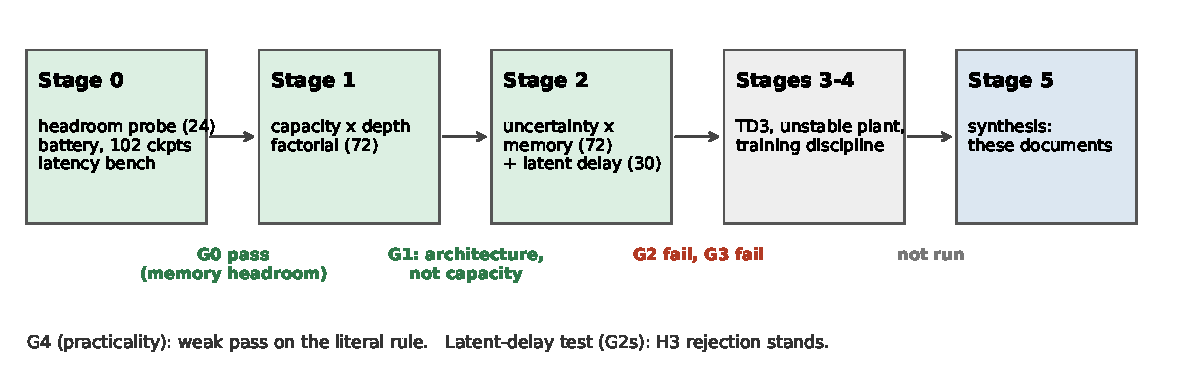
\includegraphics[width=\linewidth,height=0.42\textheight,keepaspectratio]{figures/f1_stage_map.pdf}
\caption{The Phase 3 stages and how each gate resolved}
\end{figure}



\textbf{Stage 0, and why it comes first.} Two questions, both cheap.

\begin{itemize}
\item \emph{Is there any headroom?} Before asking whether recursion can exploit uncertainty, check that uncertainty costs anything at all. A memoryless MLP was run under a fixed delay, a random delay, a random delay with the realised delay revealed (an information upper bound), and a random delay with the queue hidden.
\item \emph{What do the checkpoints we already own say?} 102 trained policies were re-evaluated with no retraining, on control-quality measures the project had never reported: command smoothness, robustness to wrong delays, sensor noise, plant changes, actuator dropout, and per-decision latency. This was the cheapest evidence in the project and it survives whatever the science does.
\end{itemize}



\textbf{A theory check that changed the design.} Working through the wrapper before submitting, one thing became clear: with a delay redrawn independently every step, every action that could reach the plant is \emph{already} in the queue, so the augmented observation is Markov. The "oracle" arm could only be a null, whether or not H3 was true. Rather than run a test that could not fail informatively, we recorded the argument, added an arm that \textbf{hides the queue} (where memory genuinely has something to reconstruct), and allowed the gate to pass on either. Everything was written down before any job ran.



\textbf{Stage 1, the attribution stage.} This is the 2$\times$2 the whole project needed: \{MLP, TRM\} $\times$ \{135k, 788k\} parameters, plus depth at fixed parameters (1, 3 and 6 outer cycles). Growing the MLP alone would only have moved the comparison to a different single capacity; shrinking TRM as well is what allows an actual attribution. The depth arm is the cleanest control in the project: \texttt{H\_cycles = 1} removes the outer recursion while changing \emph{nothing} else, not parameters, not optimiser, not inputs.



\textbf{Stage 2, the decisive stage.} Four trunks (MLP, TRM as-is, TRM carrying its latent, LSTM carrying its state) across three conditions: fixed delay with queue, random delay with queue, random delay with the queue hidden. Carrying a latent in off-policy RL is not a small change, and getting it wrong would have silently confounded the result: the behaviour policy would refine from a warm latent while the update refined from a cold one. We used stored-state replay (R2D2-style) and verified that replaying the stored carries reproduces the behaviour policy's actions exactly.



\textbf{Stages 3 and 4 were gated deliberately.} Generalisation (another algorithm, an unstable plant) and restoring TRM's training discipline only make sense if the mechanism shows \emph{something} first. Their gates did not open, so they did not run.



\textbf{One more test, added afterwards and labelled as such.} An independent review of the plan had recommended a delay drawn once per episode and held constant, which memory can identify from history, as the cleanest test of inference. We had not read that review before executing. After the main gate failed, we ran that condition too, with its rule fixed before the data. It gave the same answer.



\section*{8. What the experiments were designed to distinguish}\addcontentsline{toc}{section}{8. What the experiments were designed to distinguish}



It helps to read the whole programme as a sequence of two-way choices:



\begin{center}\small\begin{tabular}{>{\raggedright\arraybackslash}p{0.366\linewidth}>{\raggedright\arraybackslash}p{0.568\linewidth}}
\toprule
Experiment & The two explanations it separates \\
\midrule
Phase 1 (horizon/sparsity) & "recursion pays on harder tasks" vs "it doesn't" \\
Phase 2 (dimensionality, structure ablation) & "our particular recursive structure is the problem" vs "recursion in general" \\
Post-hoc re-analysis & "the environments tested the hypothesis" vs "they were floors" \\
Stage 0.1 (headroom) & "there is something to infer" vs "the input is already sufficient" \\
Stage 0.2 (battery) & "these are usable controllers" vs "they are not" \\
Stage 1 (capacity $\times$ depth) & "the deficit is size" vs "the deficit is architecture" vs "the deficit is depth" \\
Stage 2 (uncertainty $\times$ memory) & "recursion + memory exploits uncertainty" vs "it does not" \\
Latent-delay test & "memory helps when the hidden quantity is identifiable" vs "it does not" \\
\bottomrule
\end{tabular}\end{center}



\section*{9. How it came out}\addcontentsline{toc}{section}{9. How it came out}



\begin{itemize}
\item \textbf{The Phase 1 headline replicated} at higher power (12 of 12 pairs) and turned out to be \textbf{architectural, not capacity}: TRM loses to a parameter-matched MLP at both sizes, and making the MLP 5.8$\times$ bigger changes nothing.
\item \textbf{Depth is inert.} One outer cycle, three, or six make no difference to return, while cost scales with depth. That fits the gradient truncation: only 7 cell applications are ever trained.
\item \textbf{Carrying the latent changed nothing}, in any condition, even though the implementation was verified exact.
\item \textbf{Where memory had something to recover, nothing recovered it}, including when the hidden quantity was made identifiable by construction.
\item \textbf{The deficit lives in training, not in the final policy.} Run greedily, the trunks nearly tie (a 3.6-unit residual).
\item \textbf{One genuine TRM advantage:} its greedy policy is far smoother, about 0.4 torque reversals per second against the MLP's 9. It pays for that with worse robustness to noise, plant change and dropout, and with 65$\times$ the per-decision latency.
\end{itemize}



\begin{figure}[htbp]\centering
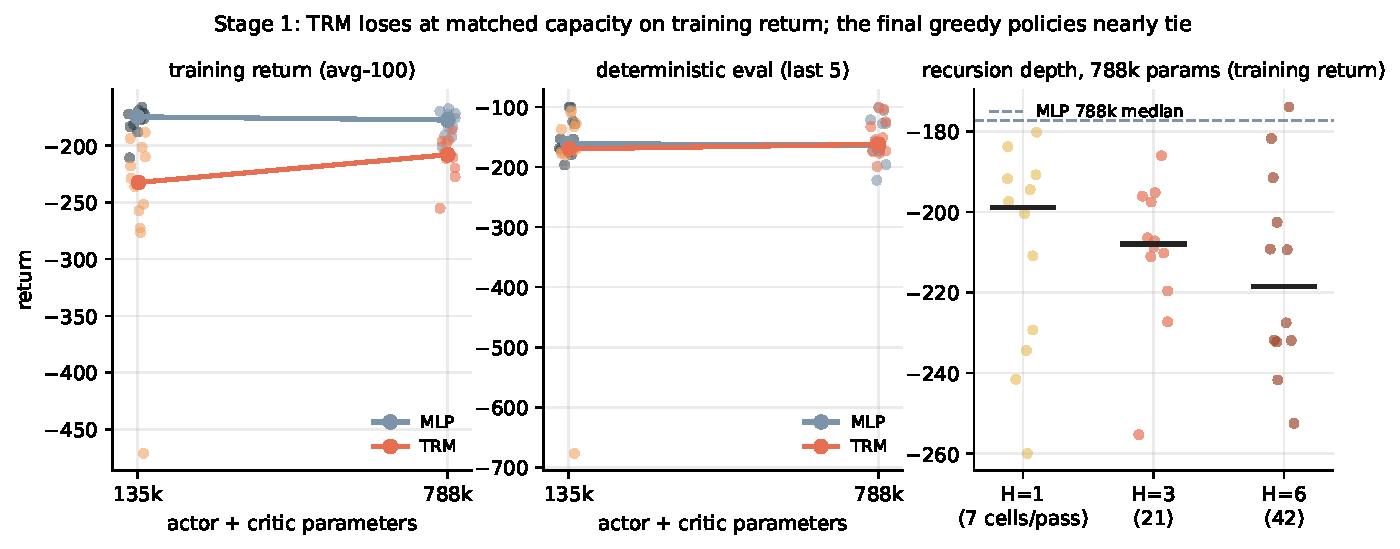
\includegraphics[width=\linewidth,height=0.42\textheight,keepaspectratio]{figures/f3_capacity_depth.pdf}
\caption{Stage 1: the deficit is architectural, and the final policies nearly tie}
\end{figure}



\textbf{The bottom line for the thesis:} this is a negative result with all three confounds removed, which is a stronger and more final claim than the Phase 1--2 draft could make. What remains open is not "does recursion help control" but "can TRM's \emph{training discipline}, not just its architecture, be ported to off-policy RL".



\medskip



\bigskip{\centering\Large\bfseries Part II --- Questions a supervisor might ask\par}\medskip\addcontentsline{toc}{section}{Part II --- Questions a supervisor might ask}



Answers are short, with the evidence attached. Where the honest answer is "we can't say", it says so.



\section*{A. Motivation and framing}\addcontentsline{toc}{section}{A. Motivation and framing}



\textbf{Q1. Why TRM at all? Why would a puzzle model be relevant to control?} Because the claim behind TRM is architectural, not task-specific: iteration with tied weights substituting for parameters. That claim, if true, matters most where parameters and compute are scarce, which is embedded control. TRM is also made of parts control already uses: a small MLP cell, applied repeatedly so that it behaves like a recurrent net. So it can be swapped in as a trunk with nothing else changed, which is what makes a like-for-like test possible.



\textbf{Q2. Why delayed control rather than, say, a harder locomotion task?} Because delay creates a principled reason for iteration to help. It breaks the Markov property; augmentation restores sufficiency in theory but says nothing about whether a small network can fit the resulting value function. Iterative refinement is a plausible inductive bias for that fitting problem. A harder locomotion task would only have varied difficulty, not the property that recursion is supposed to exploit.



\textbf{Q3. Isn't this just a negative result about your own port rather than about TRM?} After Phases 1--2, that criticism was fair, and we said so. Phase 3 was built to answer it: capacity is crossed, the latent is carried with verified stored-state replay, the conditioning is varied to where memory provably has something to reconstruct, and the environment is one where every trunk demonstrably learns. The result survives all four. What the study still cannot speak to is TRM \emph{with its training discipline} (deep supervision, no truncation), which is precisely the open question we recommend next.



\textbf{Q4. HRM-Agent already trained a recursive model with RL and it worked. Doesn't that contradict you?} No, and we cite it as the closest precedent. It succeeded on discrete mazes with a DQN head, where the task rewards multi-step planning over a revisited map. Ours is low-dimensional continuous control where a two-layer MLP already reaches the same greedy policy. Both can be true: recursion may pay where there is compositional structure to refine, and not where there isn't. HRM-Agent is also the source of the Carry-Z idea we tested.



\textbf{Q5. What is the actual contribution, in one sentence?} A confound-controlled negative: with capacity matched, the latent carried, and conditions constructed to leave something to infer, weight-tied recursion does not earn its cost in delayed model-free continuous control, and the deficit is architectural and visible in value fit rather than in final policy quality.



\section*{B. Design and method}\addcontentsline{toc}{section}{B. Design and method}



\textbf{Q6. Why DDPG? It is old and known to be brittle.} It was the algorithm the codebase was built on, and holding the learner fixed while swapping only the trunk is what makes the comparison clean. Its brittleness is a real limitation, and it explains one of our floor effects (MountainCar is a documented DDPG + OU-noise failure). TD3 support with carried state is implemented and verified; the cross-check was gated on a gate that did not open.



\textbf{Q7. Why only Pendulum for the decisive tests?} Because it is the only environment in this project where every trunk demonstrably learns within budget. Running the decisive test on a floor-effect environment is exactly the mistake Phase 2 made. The cost is external validity, and it is stated as the first limitation in all three write-ups.



\textbf{Q8. Six seeds is not many.} Agreed, and the gates are set accordingly: they detect \emph{consistent} effects, not small ones (5/6 gives one-sided p = 0.109; 12/12 pairs gives p = 0.0005). Where we had more power we used it: Stage 1 contrasts pool two conditions for n = 12, and the battery evaluates 20 episodes per checkpoint on unseen seeds. Agarwal et al.'s guidance (IQM with stratified bootstrap intervals) is applied to the evaluation results.



\textbf{Q9. Why sign tests rather than t-tests or bootstrap CIs?} Sign tests make no distributional assumption, which suits RL returns with heavy seed effects, and they were pre-registered in Phase 1 for continuity. Where distributional detail matters, the write-ups also report medians, means, per-seed differences and bootstrap intervals, so a reader can apply their own test.



\textbf{Q10. Your primary metric is training return, which includes exploration noise. Isn't that the wrong metric?} It is the metric Phases 1--2 pre-registered, so we kept it for continuity, and it is the one the gates use. But it is not the whole story, and we say so: on deterministic evaluation the same comparisons shrink from $-$34 to about $-$3.6. That distinction is itself one of the more interesting findings, because it localises the deficit to training rather than to the final controller.



\textbf{Q11. Did you tune TRM? Maybe it just needs different hyperparameters.} No, and that is a real limitation. Every trunk uses identical algorithm hyperparameters, which is what makes the swap controlled but leaves open that TRM's optimum lies elsewhere. Three things bound that concern: depth (its most obvious knob) is inert across a 6$\times$ range; capacity in both directions changes nothing; and the deficit appears in value fit, not only in return. A tuning study would be the natural rebuttal experiment, and we would run it on the shallow variant first.



\textbf{Q12. Your "capacity-matched" small TRM changes shape as well as size.} True and documented: at hidden width 44 the SwiGLU inner width rounds up to 256, so its expansion ratio differs from the 128-wide trunk. That is why the attribution rests on \emph{both} directions of the 2$\times$2 (shrinking TRM and growing the MLP) plus the depth arm, rather than on a single cell.



\textbf{Q13. The carried LSTM was not tuned. Doesn't that weaken the memory comparison?} Yes, and we flag it in the limitations of all three documents. It is engineered correctly (the same verified stored-state machinery as Carry-Z) but untuned, so "Carry-Z beats the LSTM" is not evidence for recursion. The load-bearing memory comparison is Carry-Z vs Reset-Z, which are identical networks differing only in whether the latent persists.



\textbf{Q14. How do you know Carry-Z is implemented correctly?} By a reproduction check rather than by inspection. Feeding the stored carries back through the networks reproduces the behaviour policy's actions and its next carries with \textbf{zero error}, for both actor and critic. Carry-Z also has exactly the same parameter count as Reset-Z in every condition, so nothing else moved.



\textbf{Q15. How do you know the delay wrapper does what you claim?} Every extension was checked to be \textbf{bit-identical} to the original wrapper on all pre-existing delay and augmentation configurations, so no earlier result changed underneath us. The new behaviours were tested directly: exact discrete-uniform sampling, the oracle value matching the realised delay every step, and the per-episode delay staying constant within an episode and varying across episodes.



\section*{C. Results and interpretation}\addcontentsline{toc}{section}{C. Results and interpretation}



\textbf{Q16. What is the headline number?} On Pendulum-v1, TRM trails a parameter-matched MLP at both capacities: $-$50.2 at 135k (0/12 pairs) and $-$27.1 at 788k (2/12). Against the original small MLP it is $-$34.4 (0/12, p = 0.0005), reproducing Phase 1's $-$32.8 at higher power.



\textbf{Q17. Is a 34-unit difference practically meaningful?} Barely, on its own: it is about 3\% of the span between an untrained policy ($\approx$ $-$1460) and the best result seen. Two things make it matter anyway. It is \emph{perfectly consistent} (0/12), and it comes with an 11--13$\times$ training cost and a 65$\times$ latency cost. At matched wall-clock rather than matched episodes, the gap is not 3\% but most of the span: when the MLP finishes, TRM has completed 16 of 200 episodes.



\textbf{Q18. Why is the value fit worse? What is the mechanism?} We can say what it is not: it is not capacity (a 5.8$\times$ bigger MLP fits slightly \emph{better}), and it is not depth (the deficit narrows when the outer recursion is removed entirely). What remains is the recursive cell itself as trained here. The most plausible account is the truncation: only 7 of 21 applications receive gradient, so the extra computation is untrained transformation layered on a single trained pass. That account predicts depth inertness, which we observe.



\textbf{Q19. Depth is inert. Isn't that evidence you implemented TRM wrongly?} It is evidence that the \emph{ported} recursion does nothing here, which is the finding. It also matches in-domain analyses of TRM and HRM: most accuracy arrives at the first recursion step, training-time refinement dominates inference-time depth, and removing the per-instance identity collapses accuracy. Those components are exactly what a model-free RL port cannot carry over.



\textbf{Q20. You found TRM is smoother. Is that a real effect or noise?} Real at the power we have, and it was not visible at lower power. Across 12 paired Stage 1 checkpoints, TRM's greedy policy reverses torque direction about 0.4 times per second against the MLP's 9, with fewer reversals in 11 of 12 pairs (p = 0.006), at a final return only 3.6 units lower. With only 3 seeds (the banked checkpoints) it sat inside seed noise, because one TRM seed chattered. It is also not a depth effect (H = 1 and H = 3 are indistinguishable), so it appears to come from the cell, plausibly an implicit smoothness prior from the normalised, weight-tied update.



\textbf{Q21. Then is TRM actually better for actuator wear?} It is a trade, and we present it that way. It buys smoothness at the price of robustness: under sensor noise it loses 76 more reward units than the MLP (2/12 favourable, p = 0.039), and it degrades more under a 30\% heavier pendulum and under 10\% actuator dropout, with the deepest variant worst. For a benign environment where actuator wear dominates, the trade could be worth it; for this project's delay-robustness brief, it is not.



\textbf{Q22. Why did revealing the delay make the MLP \emph{worse}?} Because under an independently redrawn delay the realised past delay carries no information about the next one, while still adding an input dimension the network must learn to ignore. We predicted this before running it, which is why the headroom gate was amended to pass on the queue-hiding contrast instead.



\textbf{Q23. In Stage 2 the resetting TRM beat the MLP at one condition. Doesn't that support recursion?} No, and we report it as an exploratory observation with its likely cause. That condition is the one where the extra previous-action input \emph{hurt} the MLP ($-$63.7, 1/6 paired against an otherwise identical arm without it). And H3 cannot produce that result: the condition has nothing to infer and the resetting trunk has no memory.



\textbf{Q24. In the latent-delay test, the interaction you predicted appears in 5 of 6 seeds. Why not claim it?} Because the same pattern appears \emph{more strongly} for the trunk with no memory at all (+53.0 vs +15.1), which rules out the mechanism H3 proposes. Its actual cause is the MLP collapsing in two seeds under that delay (seed SD 169 against 32--33 for either TRM). The real observation is that the recursive trunks train more \emph{consistently} there, which is about optimisation stability, not inference, and we label it exploratory.



\textbf{Q25. Your amendment A-6 gave every trunk its previous action, and that removed most of the headroom. Did you undermine your own decisive test?} Partly, and we disclose it: with that input, the memoryless MLP recovers most of what hiding the queue took away (+67.0, 5/6). The conclusion does not depend on it, because Carry-Z also fails to beat a \emph{history-free} MLP from Stage 0 at the same condition ($-$19.2, 2/6). If I ran Stage 2 again I would include both input variants as a factor rather than fixing it.



\section*{D. Validity, rigour and process}\addcontentsline{toc}{section}{D. Validity, rigour and process}



\textbf{Q26. How do I know you didn't fish for these results?} Every decision rule was written down before its data, in a file with timestamps, and the write-ups report the rules verbatim alongside the outcomes. Two things follow from that discipline and are reported honestly rather than quietly fixed: the originally pre-registered headroom contrast \textbf{failed} and only the amended one passed, and the practicality gate passed in a degenerate way (an untrained LSTM satisfies "smooth at matched return"). We report the rule as written and name the degenerate pass.



\textbf{Q27. But you did amend the plan. Isn't that moving the goalposts?} The amendments were recorded before any Stage 0 job ran, and they are additive: every originally pre-registered arm still ran and is still reported. The amendment exists because a theory check showed one arm could not be informative. The later latent-delay test is the one thing that came after a gate failed; its rule was fixed before its data and it is labelled supplementary everywhere it appears.



\textbf{Q28. Why did you stop at Stage 2 instead of running Stages 3 and 4?} Because their entry conditions are pre-registered and did not open. Stage 3 asks whether a finding generalises, and there was no finding to generalise. Stage 4 asks whether restoring the training discipline recovers a benefit, and its gate (does carrying the latent do anything at all?) failed. Running them anyway would have turned a confirmatory programme into an exploratory one, and would have spent GPU time to weaken the claim rather than strengthen it.



\textbf{Q29. Would Stage 4 change your conclusion if you ran it?} It could, and that is exactly why the conclusion is scoped to "recursion as ported, without TRM's training discipline". If supervising every cycle or removing the truncation recovered a benefit, the finding would become "the discipline, not the architecture, is what transfers", which is a positive result worth having. I would run it as exploration, and I would pair it with a tuning sweep.



\textbf{Q30. How many comparisons did you run? Should there be a multiple-comparison correction?} The gates are single pre-registered statistics, one per stage, which is the protection against multiplicity for the confirmatory claims. The write-ups do report many secondary contrasts, and those are labelled secondary or exploratory; none carries a confirmatory claim. Where two conditions were co-primary (C3 and C4), both are reported whatever they show.



\textbf{Q31. Is the study reproducible?} Yes, more so than the earlier phases. Every stage ran from a frozen code snapshot, each job's results file embeds its full resolved configuration and its GPU model, and a bug from Phases 1--2 was fixed along the way: the warmup actions were unseeded, so those runs could not be reproduced exactly. They are now seeded from the run seed, and every arm's first episode is identical as a result.



\textbf{Q32. What went wrong operationally, and how do I know it didn't corrupt results?} Three things, all recorded. Five jobs landed on a GPU architecture the installed PyTorch has no kernels for; they crashed loudly and were rerouted and rerun. A queue-tier change required deleting and resubmitting 46 queued jobs from the same frozen snapshot. And the evaluation battery skipped six checkpoints whose result filenames collided; they were identified by checkpoint ID and evaluated separately. Nothing produced silent wrong numbers: the first two fail loudly, and the third was caught by a file count.



\textbf{Q33. Hardware varied across runs. Does that affect the cost claims?} Training times are compared only within a GPU model (10.8$\times$ on A100, 11.7$\times$ on L40S, 13.0$\times$ on V100), and every result records its device. The latency benchmark ran on one fixed machine, one CPU thread and one A100.



\section*{E. Bigger picture and next steps}\addcontentsline{toc}{section}{E. Bigger picture and next steps}



\textbf{Q34. What is the single most important thing you learned?} That the interesting question moved. It started as "does recursion beat an MLP?" and ended as "what part of TRM was actually doing the work?" The answer the evidence points to is: not the forward-pass depth, which is inert here, but the training discipline around it, which a model-free RL port cannot carry over.



\textbf{Q35. What would you do differently?} Three things. Validate the environment ladder with a budget pilot \emph{before} committing a matrix, which is what caused two floor-effect phases. Read the plan review before executing rather than after, which would have made the latent-delay condition primary instead of supplementary. And build the previous-action input in as a factor rather than fixing it across all arms.



\textbf{Q36. What would falsify your conclusion?} Any of: a tuned TRM beating a tuned MLP at matched capacity on a validated environment; the training-discipline variants (no truncation, per-cycle supervision) recovering the gap; or a carried-latent trunk exploiting delay uncertainty where a memoryless one provably cannot. The last of these is the test we sharpened most, and it came back negative twice.



\textbf{Q37. What next, if you had three more months?} In order: (1) restore TRM's training discipline, because it is the one route left to a constructive positive; (2) generalise the negative with TD3 and an open-loop-unstable plant, using a budget pilot first (both are built and unused); (3) re-test the original complexity-scaling question on environments that are actually learned; (4) a tuned recurrent baseline before any further claim about memory.



\textbf{Q38. Is there anything here worth publishing on its own?} Three candidates. The confound-controlled negative itself, which is the kind of result that saves other people compute. The depth-inertness and value-fit result, which connects to independent analyses of TRM and HRM from outside RL. And the smoothness-versus-robustness trade, which is a control-engineering observation the RL-architecture literature rarely measures at all.



\textbf{Q39. If someone wants to build on this, what do they need?} The plan and its amendments (\texttt{papers/\allowbreak{}phase3/\allowbreak{}plan.\allowbreak{}md}), the gate rules as they were fixed (\texttt{experiments/\allowbreak{}phase3/\allowbreak{}dashboard\_\allowbreak{}state/\allowbreak{}gates.\allowbreak{}json}), the analysis outputs (\texttt{experiments/\allowbreak{}analysis\_\allowbreak{}*.\allowbreak{}json}), and the raw runs (\texttt{results\_\allowbreak{}phase3/\allowbreak{}}, with checkpoints on Katana). Every figure in the write-ups regenerates from one script, and each document's PDF builds from its Markdown source.



\medskip



\section*{Appendix --- Numbers worth memorising}\addcontentsline{toc}{section}{Appendix --- Numbers worth memorising}



\begin{center}\small\begin{tabular}{>{\raggedright\arraybackslash}p{0.387\linewidth}>{\raggedright\arraybackslash}p{0.547\linewidth}}
\toprule
Fact & Number \\
\midrule
Phase 1 headline (TRM $-$ MLP, Pendulum) & $-$37.1; 0/6 seed pairs; p = 0.016 \\
Same contrast in Stage 1 & $-$34.4; 0/12 pairs; p = 0.0005 \\
TRM vs matched MLP (135k / 788k) & $-$50.2 (0/12) / $-$27.1 (2/12) \\
Effect of MLP capacity (788k vs 135k) & $-$3.8; 5/12 (nothing) \\
Depth (H = 1 / H = 6 vs H = 3) & $-$3.3 (5/12) / $-$10.9 (4/12) \\
Value fit at matched capacity (late) & 1.45$\times$ and 1.89$\times$; 12/12 each \\
Deterministic final-policy gap & $-$3.6; 2/12; p = 0.039 \\
Memory headroom (queue hidden) & 70.8; 6/6; p = 0.016 \\
G2 interaction at the decisive condition & $-$40.0; 1/6 (wrong sign) \\
Carry-Z vs Reset-Z (C1 / C3 / C4 / C6) & +4.8 / $-$22.0 / +16.7 / $-$4.9; never $\geq$ 5/6 \\
Torque reversals per second (TRM vs MLP) & 0.38 vs 9.06; 11/12 pairs; p = 0.006 \\
Sensor-noise penalty vs MLP & $-$75.8; 2/12; p = 0.039 \\
Decision latency, 1 CPU thread (p99) & 0.064 ms vs 4.13 ms (65$\times$); 242 Hz ceiling \\
Training cost, same GPU & 11--13$\times$ (H = 6: 18--24$\times$) \\
Totals & 300 training runs; 300 checkpoint evaluations; 231 Phase 3 jobs \\
\bottomrule
\end{tabular}\end{center}



\begin{figure}[htbp]\centering
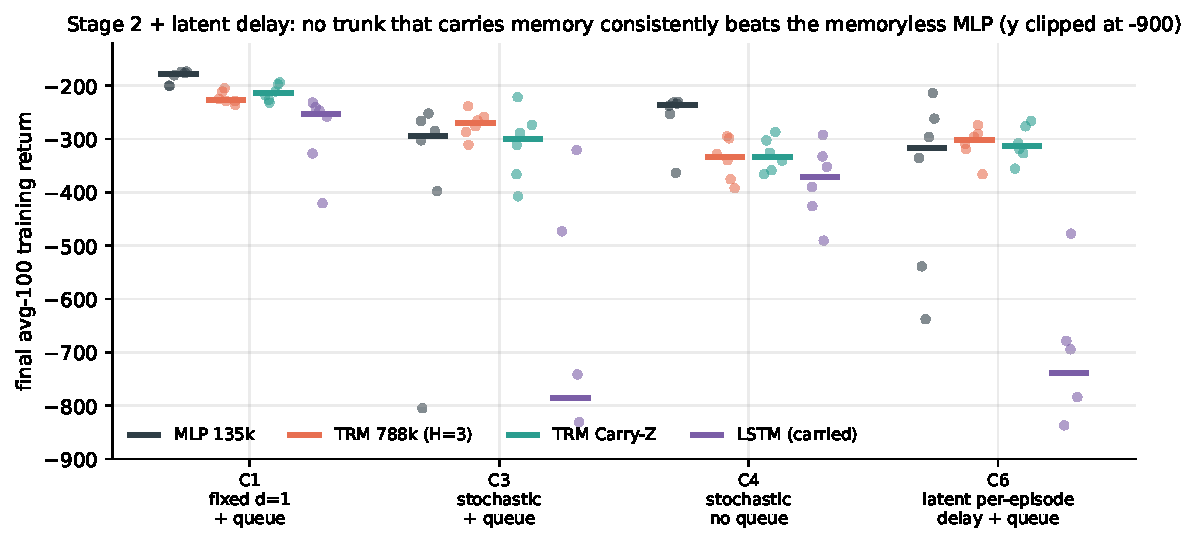
\includegraphics[width=\linewidth,height=0.42\textheight,keepaspectratio]{figures/f5_stage2.pdf}
\caption{Stage 2 and the latent-delay condition: no memory-carrying trunk consistently beats the memoryless MLP}
\end{figure}



\begin{figure}[htbp]\centering
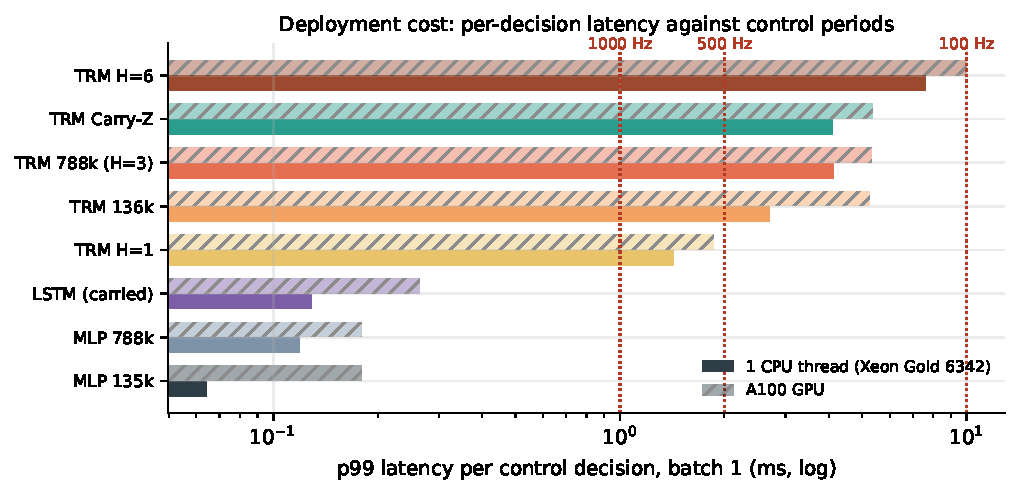
\includegraphics[width=\linewidth,height=0.42\textheight,keepaspectratio]{figures/f6_latency.pdf}
\caption{Per-decision latency against control periods}
\end{figure}
\end{document}
